\begin{figure}[H]
  \centering
  \begin{minipage}[b]{0.45\textwidth}
    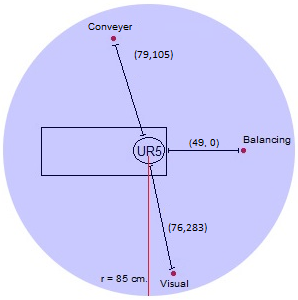
\includegraphics[width=\textwidth]{Design/workcell_1_polar.png}
    \label{fig:position}
  \end{minipage}
  \hfill
  \begin{minipage}[b]{0.45\textwidth}
    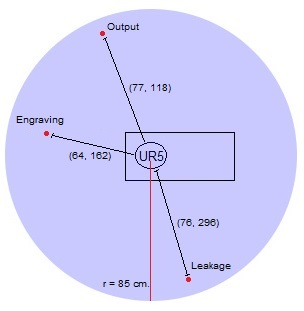
\includegraphics[width=\textwidth]{Design/polar.jpg}  
    \label{fig:velocity}
  \end{minipage}
  {Work-cell first and second part ,with polar coordinates and reach to suited the reach of the UR 5.}
  \label{fig:firstpart}
\end{figure}

%Flowchart 1:
%\begin{tikzpicture}[node distance=2cm]

%Primary nodes:
%\node (start) [startstop] {Rotor arrives on conveyer/queue table};
%\node (dec1) [decision, below of=start, yshift=-2.5cm] {Has this rotor been balance tested?};
%\node (dec2) [decision, right of=dec1, xshift=3.2cm] {Is the balancing
%machine empty?};
%\node (pro1) [process, right of=dec2, xshift=3.1cm] {Move the rotor to balancing machine};
%\node (out1) [io, below of=pro1, yshift=-3cm] {Balancing complete};
%\node (dec3) [decision, below of=dec1, yshift=-6cm] {Has this %rotor been visually inspected?};
%\node (dec4) [decision, right of=dec3, xshift=3.2cm] {Is %visual inspection available?};
%\node (pro2) [process, right of=dec4, xshift=3.1cm] {Move the %rotor to visual inspection};
%\node (out2) [io, below of=pro2, yshift=-3cm] {Visual %inspection complete};
%\node (stop) [startstop, below of=dec3, yshift=-5cm] {Move %rotor to queue table};

%Primary arrows:
%\draw [arrow] (start) -- (dec1);
%\draw [arrow] (dec1) -- node[anchor=south] {no} (dec2);
%\draw [arrow] (dec1) -- node[anchor=west] {yes} (dec3);
%\draw [arrow] (dec2) -- node[anchor=south] {yes} (pro1);
%\draw [arrow] (pro1) -- (out1);
%\draw [arrow] (dec3) -- node[anchor=south] {no} (dec4);
%\draw [arrow] (dec3) -- node[anchor=west]  {yes} (stop);
%\draw [arrow] (dec4) -- node[anchor=south] {yes} (pro2);
%\draw [arrow] (pro2) -- (out2);

%dec2, dec4 -> start:
%\node (gui1) [Guidebox, left of=pro1, xshift=-11cm] {};
%\node (gui2) [Guidebox, below of=gui1, yshift=-0.85cm] {};
%\node (gui6) [Guidebox, left of=pro2, xshift=-11cm] {};
%\node (gui7) [Guidebox, below of=gui6, yshift=-0.85cm] {};

%Below dec2:
%\node (gui3) [Guidebox, right of=gui2, xshift=5.9cm] {};
%\node (gui4) [Guidebox, below of=gui3, yshift=1.9cm] {};
%\node (gui5) [Guidebox, right of=gui3, xshift=-1.9cm] {};
%\draw [arrow] (dec2) -- node[anchor=west] {no} (gui4);
%\draw [arrow] (gui5) -- (gui2);

%Below dec4:
%\node (gui8) [Guidebox, right of=gui7, xshift=5.9cm] {};
%\node (gui9) [Guidebox, below of=gui8, yshift=1.9cm] {};
%\node (gui10) [Guidebox, right of=gui8, xshift=-1.9cm] {};
%\draw [arrow] (dec4) -- node[anchor=west] {no} (gui9);

%Line to start:
%\node (gui11) [Guidebox, above of=gui1, yshift=2.55cm] {};
%\node (gui12) [Guidebox, above of=gui11, yshift=-1.9cm] {};
%\node (gui13) [Guidebox, left of=gui11, xshift=1.9cm] {};
%\node (gui16) [Guidebox, below of=gui7, yshift=1.9cm] {};
%\node (gui17) [Guidebox, left of=gui7, xshift=1.9cm] {};
%\draw [arrow] (gui10) -- (gui17);
%\draw [arrow] (gui16) -- (gui12);
%\draw [arrow] (gui13) -- (start);

%out1, out2 -> dec3, stop:
%\node (gui14) [Guidebox, above of=dec3, yshift=1cm] {};
%\draw [arrow] (out1) -- (gui14);
%\node (gui15) [Guidebox, above of=stop, yshift=-0cm] {};
%\draw [arrow] (out2) -- (gui15);

%Caption:
%\node (cap1) [Caption, below of=dec4, yshift=-7cm] {This %flowchart shows the process performed by the first UR5 in the %work-cell.};

%\label{fig:first-part}
%\end{tikzpicture}


%Flowchart 2:
%\begin{tikzpicture}[node distance=2cm]

%%Primary nodes:
%\node (start) [startstop] {Rotor arrives on queue-table};
%\node (dec1) [decision, below of=start, yshift=-2.5cm] {Has %this rotor been leak tested?};
%\node (dec2) [decision, right of=dec1, xshift=3.2cm] {Is the %leak testing
%machine empty?};
%\node (pro1) [process, right of=dec2, xshift=3.1cm] {Move the %rotor to leak testing machine};
%\node (out1) [io, below of=pro1, yshift=-3cm] {Leak testing %complete};
%\node (dec3) [decision, below of=dec1, yshift=-6cm] {Has this rotor been engraved?};
%\node (dec4) [decision, right of=dec3, xshift=3.2cm] {Is the engraving
%machine empty?};
%\node (pro2) [process, right of=dec4, xshift=3.1cm] {Move the rotor to engraving machine};
%\node (out2) [io, below of=pro2, yshift=-3cm] {Engraving complete};
%\node (stop) [startstop, below of=dec3, yshift=-5cm] {Move rotor to output pallet};

%Primary arrows:
%\draw [arrow] (start) -- (dec1);
%\draw [arrow] (dec1) -- node[anchor=south] {no} (dec2);
%\draw [arrow] (dec1) -- node[anchor=west] {yes} (dec3);
%\draw [arrow] (dec2) -- node[anchor=south] {yes} (pro1);
%\draw [arrow] (pro1) -- (out1);
%\draw [arrow] (dec3) -- node[anchor=south] {no} (dec4);
%\draw [arrow] (dec3) -- node[anchor=west]  {yes} (stop);
%\draw [arrow] (dec4) -- node[anchor=south] {yes} (pro2);
%\draw [arrow] (pro2) -- (out2);

%dec2, dec4 -> start:
%\node (gui1) [Guidebox, left of=pro1, xshift=-11cm] {};
%\node (gui2) [Guidebox, below of=gui1, yshift=-0.85cm] {};
%\node (gui6) [Guidebox, left of=pro2, xshift=-11cm] {};
%\node (gui7) [Guidebox, below of=gui6, yshift=-0.85cm] {};

%Below dec2:
%\node (gui3) [Guidebox, right of=gui2, xshift=5.9cm] {};
%\node (gui4) [Guidebox, below of=gui3, yshift=1.9cm] {};
%\node (gui5) [Guidebox, right of=gui3, xshift=-1.9cm] {};
%\draw [arrow] (dec2) -- node[anchor=west] {no} (gui4);
%\draw [arrow] (gui5) -- (gui2);

%Below dec4:
%\node (gui8) [Guidebox, right of=gui7, xshift=5.9cm] {};
%\node (gui9) [Guidebox, below of=gui8, yshift=1.9cm] {};
%\node (gui10) [Guidebox, right of=gui8, xshift=-1.9cm] {};
%\draw [arrow] (dec4) -- node[anchor=west] {no} (gui9);

%Line to start:
%\node (gui11) [Guidebox, above of=gui1, yshift=2.55cm] {};
%\node (gui12) [Guidebox, above of=gui11, yshift=-1.9cm] {};
%\node (gui13) [Guidebox, left of=gui11, xshift=1.9cm] {};
%\node (gui16) [Guidebox, below of=gui7, yshift=1.9cm] {};
%\node (gui17) [Guidebox, left of=gui7, xshift=1.9cm] {};
%\draw [arrow] (gui10) -- (gui17);
%\draw [arrow] (gui16) -- (gui12);
%\draw [arrow] (gui13) -- (start);

%out1, out2 -> dec3, stop:
%\node (gui14) [Guidebox, above of=dec3, yshift=1cm] {};
%\draw [arrow] (out1) -- (gui14);
%\node (gui15) [Guidebox, above of=stop, yshift=-0cm] {};
%\draw [arrow] (out2) -- (gui15);

%Caption:
%\node (cap1) [Caption, below of=dec4, yshift=-7cm] {This flowchart shows the process performed by the second UR5 in the work-cell.};

%\end{tikzpicture}

The following flowcharts show the different processes performed by the 2 robots in the work cell. The red box in each flow chart shows which events trigger the program, which the flowchart represents. The green rhombuses are decisions, which can lead to different outcomes. The yellow boxes are the tasks, which the robots will perform. The black dots are signals, which are sent to the robots by the machines. The blue boxes are signals, which are sent to the robots by other sources. 

%Flowchart 1:
\begin{tikzpicture}[node distance=2cm]

%Primary nodes:
\node (start) [startstop] {Rotor arrives $\vee$ visual done};
\node (dec1) [decision, below of=start, yshift=-2cm] {Is the balancing machine empty, and is a rotor available?};
\node (pro1) [process, below of=dec1, yshift=-2.5cm] {Place rotor in the balancing machine};
\node (dot1) [Blackdot, below of=pro1, yshift=-0.5cm] {};

%Primary arrows:
\draw [arrow] (start) -- (dec1);
\draw [arrow] (dec1) -- node[anchor=west] {yes} (pro1);
\draw [arrow] (pro1) -- (dot1);

%Guideboxes: 
\node (gui1) [Guidebox, left of=dec1, xshift=-1.25cm] {};
\node (gui2) [Guidebox, above of=gui1, yshift=-1.9cm] {};
\node (gui3) [Guidebox, left of=gui1, xshift=1.9cm] {};
\draw [arrow] (dec1) -- node[anchor=south] {no} (gui3);

\node (gui4) [Guidebox, left of=dot1, xshift=-1.25cm] {};
\node (gui5) [Guidebox, below of=gui4, yshift=1.9cm] {};
\node (gui6) [Guidebox, left of=gui4, xshift=1.9cm] {};
\draw [arrow] (gui6) -- (dot1);

\draw [arrow] (gui2) -- (gui5);

%Flowchart2:

%Primary nodes: 
\node (start2) [startstop, right of=start, xshift=5cm] {Balancing done};
\node (dec3) [decision, below of=start2, yshift=-1.5cm] {Did the rotor fail balancing?};
\node (pro3) [process, below of=dec3, yshift=-2cm] {Move rotor to visual inspection};
\node (dec4) [decision, below of=pro3, yshift=-2cm] {Did the rotor pass visual inspection?};
\node (pro4) [process, below of=dec4, yshift=-2cm] {Move rotor to queue table};
\node (stop2) [io, below of=pro4, yshift=-0.5cm] {Visual done};


%Primary arrows:
\draw [arrow] (start2) -- (dec3);
\draw [arrow] (dec3) -- node[anchor=west] {no} (pro3);
\draw [arrow] (pro3) -- (dec4);
\draw [arrow] (dec4) -- node[anchor=west] {yes} (pro4);
\draw [arrow] (pro4) -- (stop2);

%Guideboxes: 
\node (gui11) [Guidebox, left of=dec3, xshift=-2cm] {};
\node (gui12) [Guidebox, above of=gui11, yshift=-1.9cm] {};
\node (gui13) [Guidebox, left of=gui11, xshift=1.9cm] {};
\draw [arrow] (dec3) -- node[anchor=south] {yes} (gui13);

\node (gui14) [Guidebox, left of=dec4, xshift=-2cm] {};
\node (gui15) [Guidebox, above of=gui14, yshift=-1.9cm] {};
\node (gui16) [Guidebox, left of=gui14, xshift=1.9cm] {};
\draw [arrow] (dec4) -- node[anchor=south] {no} (gui16);

\node (gui17) [Guidebox, left of=stop2, xshift=-2cm] {};
\node (gui18) [Guidebox, below of=gui17, yshift=1.9cm] {};
\node (gui19) [Guidebox, left of=gui17, xshift=1.9cm] {};
\draw [arrow] (gui19) -- (stop2);

\draw [arrow] (gui12) -- (gui18);

\node (out1) [process, above of=gui18, yshift=0.75cm] {Move rotor to failed pile};

%Caption:
\node (cap1) [Caption, below of=gui19, yshift=-2cm] {These event based flowcharts show the process performed by the first UR5 in the work-cell.};

\end{tikzpicture}









%Flowchart 3:
\begin{tikzpicture}[node distance=2cm]

%Primary nodes:
\node (start) [startstop] {Rotor arrives $\vee$ Output done};
\node (dec1) [decision, below of=start, yshift=-2cm] {Is the leakage testing machine empty, and is a rotor available?};
\node (pro1) [process, below of=dec1, yshift=-2.7cm] {Place rotor in the leakage testing machine};
\node (dot1) [Blackdot, below of=pro1, yshift=-0.5cm] {};

%Primary arrows:
\draw [arrow] (start) -- (dec1);
\draw [arrow] (dec1) -- node[anchor=west] {yes} (pro1);
\draw [arrow] (pro1) -- (dot1);

%Guideboxes: 
\node (gui1) [Guidebox, left of=dec1, xshift=-1.25cm] {};
\node (gui2) [Guidebox, above of=gui1, yshift=-1.9cm] {};
\node (gui3) [Guidebox, left of=gui1, xshift=1.9cm] {};
\draw [arrow] (dec1) -- node[anchor=south] {no} (gui3);

\node (gui4) [Guidebox, left of=dot1, xshift=-1.25cm] {};
\node (gui5) [Guidebox, below of=gui4, yshift=1.9cm] {};
\node (gui6) [Guidebox, left of=gui4, xshift=1.9cm] {};
\draw [arrow] (gui6) -- (dot1);

\draw [arrow] (gui2) -- (gui5);


%Flowchart 4:

%Primary nodes:
\node (start2) [startstop, right of=start, xshift=5cm] {Engraving done};
\node (dec2) [decision, below of=start2, yshift=-1.5cm] {Is the engraving process complete?};
\node (pro2) [process, below of=dec2, yshift=-2.5cm] {Move rotor from engraving machine to output pallet};
\node (stop2) [io, below of=pro2, yshift=-0.5cm] {Output done}; 

%Primary arrows:
\draw [arrow] (start2) -- (dec2);
\draw [arrow] (dec2) -- node[anchor=west] {yes} (pro2);
\draw [arrow] (pro2) -- (stop2);

%Guideboxes: 
\node (gui11) [Guidebox, left of=dec2, xshift=-1.25cm] {};
\node (gui12) [Guidebox, above of=gui11, yshift=-1.9cm] {};
\node (gui13) [Guidebox, left of=gui11, xshift=1.9cm] {};
\draw [arrow] (dec2) -- node[anchor=south] {no} (gui13);

\node (gui14) [Guidebox, left of=stop2, xshift=-1.25cm] {};
\node (gui15) [Guidebox, below of=gui14, yshift=1.9cm] {};
\node (gui16) [Guidebox, left of=gui14, xshift=1.9cm] {};
\draw [arrow] (gui16) -- (stop2);

\draw [arrow] (gui12) -- (gui15);

%Caption:
\node (cap1) [Caption, below of=gui16, yshift=-2cm] {These event based flowcharts show a part of the process performed by the second UR5 in the work-cell.};


\end{tikzpicture}









%Flowchart 5:
\begin{tikzpicture}[node distance=2cm]

%Primary nodes:
\node (start) [startstop] {Leakage testing done};
\node (dec1) [decision, below of=start, yshift=-1.5cm] {Did the rotor fail leakage testing?};
\node (pro1) [process, below of=dec1, yshift=-2.5cm] {Move rotor to engraving machine};
\node (dot1) [Blackdot, below of=pro1, yshift=-0.5cm] {};

%Primary arrows:
\draw [arrow] (start) -- (dec1);
\draw [arrow] (dec1) -- node[anchor=west] {no} (pro1);
\draw [arrow] (pro1) -- (dot1);

%Guideboxes: 
\node (gui1) [Guidebox, left of=dec1, xshift=-2cm] {};
\node (gui2) [Guidebox, above of=gui1, yshift=-1.9cm] {};
\node (gui3) [Guidebox, left of=gui1, xshift=1.9cm] {};
\draw [arrow] (dec1) -- node[anchor=south] {yes} (gui3);

\node (gui4) [Guidebox, left of=dot1, xshift=-2cm] {};
\node (gui5) [Guidebox, below of=gui4, yshift=1.9cm] {};
\node (gui6) [Guidebox, left of=gui4, xshift=1.9cm] {};
\draw [arrow] (gui6) -- (dot1);

\draw [arrow] (gui2) -- (gui5);

\node (out1) [process, above of=gui5, yshift=0.75cm] {Move rotor to failed pile};

%Caption:
\node (cap1) [Caption, below of=dot1, yshift=-2cm] {This event based flowchart shows a part of the process performed by the second UR5 in the work-cell.};

\end{tikzpicture}



